\subsection{Receipt Evidence-Context Controls}
\label{sec:eval:recovery_ablation}
We compare six contexts on the same 60 frozen follow-up receipts using 360
new Gemma responses, collected with the factorial controls. All responses
parse successfully. Each arm retains the full source and shares the model,
output budget, and filter. The random index approximately matches index
character length; it does not match token count exactly. These are repeated
measurements on the same documents, not a new independent test set.

\begin{table}[t]

\centering

\caption{Receipt context controls with the same model, source and output budget. All rows include the same filter; sixty documents per row. Random context approximately matches index character length, not exact token count.}

\label{tab:recovery_index}

\small

\begin{tabular}{lrr}

\toprule

Context & Exact F1 & Normalized F1 \\

\midrule

Simple & 0.7917 & 0.8125 \\

Full index & 0.8351 & 0.8643 \\

Anchors only & 0.8351 & 0.8643 \\

Random index & 0.8167 & 0.8458 \\

Simple, no definitions & 0.8083 & 0.8292 \\

Full index, no definitions & 0.7470 & 0.7762 \\

\bottomrule

\end{tabular}

\end{table}

The full index leads Simple by 4.35 F1 points (95\% CI: 1.25 to 7.86), but the contrast has $p_H=0.065$ across the five prespecified comparisons. Full and anchors-only have identical mean F1; full minus random is 1.85 points (CI: $[-0.65,4.52]$, $p_H=0.696$). Removing field definitions from the full index lowers F1 by 8.81 points (CI: $[4.23,13.39]$, $p_H=0.006$), whereas definitions do not improve the simple arm in this batch. These controls support the combination of field definitions and indexed context, while leaving the added value of neighbouring lines and targeted rather than random context unresolved.

\begin{figure}[t]

\centering

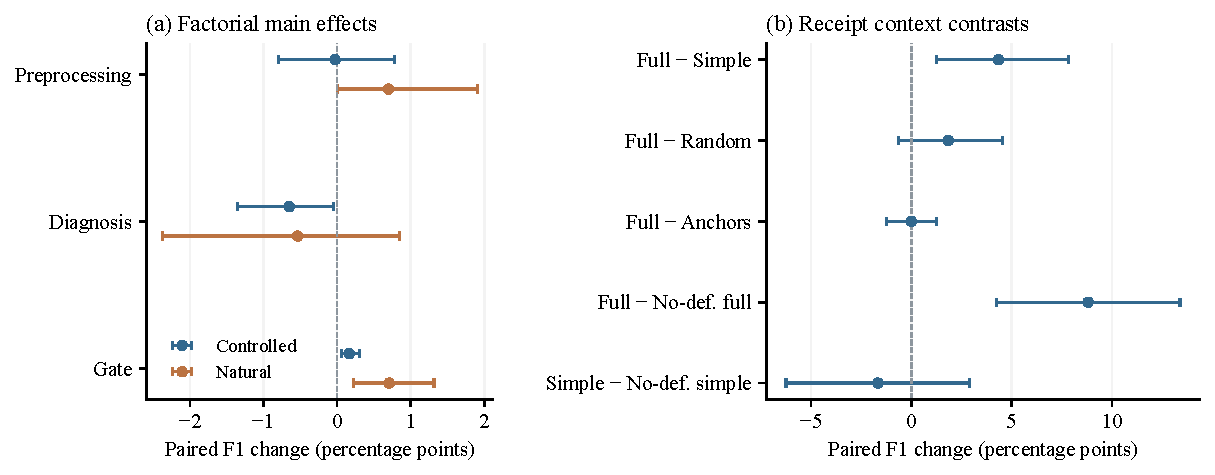
\includegraphics[width=0.98\textwidth]{figure/experiments/recovery_ablation.pdf}

\caption{Contemporaneous factorial and receipt-context controls. Points show paired mean F1 differences and bars show marginal 95\% document-bootstrap intervals. Main-effect and receipt-contrast families receive separate Holm corrections; intervals are not multiplicity-adjusted.}

\label{fig:recovery_ablation}

\end{figure}
